% Options for packages loaded elsewhere
\PassOptionsToPackage{unicode}{hyperref}
\PassOptionsToPackage{hyphens}{url}
\PassOptionsToPackage{dvipsnames,svgnames,x11names}{xcolor}
%
\documentclass[
]{interact}

\usepackage{amsmath,amssymb}
\usepackage{setspace}
\usepackage{iftex}
\ifPDFTeX
  \usepackage[T1]{fontenc}
  \usepackage[utf8]{inputenc}
  \usepackage{textcomp} % provide euro and other symbols
\else % if luatex or xetex
  \usepackage{unicode-math}
  \defaultfontfeatures{Scale=MatchLowercase}
  \defaultfontfeatures[\rmfamily]{Ligatures=TeX,Scale=1}
\fi
\usepackage{lmodern}
\ifPDFTeX\else  
    % xetex/luatex font selection
\fi
% Use upquote if available, for straight quotes in verbatim environments
\IfFileExists{upquote.sty}{\usepackage{upquote}}{}
\IfFileExists{microtype.sty}{% use microtype if available
  \usepackage[]{microtype}
  \UseMicrotypeSet[protrusion]{basicmath} % disable protrusion for tt fonts
}{}
\makeatletter
\@ifundefined{KOMAClassName}{% if non-KOMA class
  \IfFileExists{parskip.sty}{%
    \usepackage{parskip}
  }{% else
    \setlength{\parindent}{0pt}
    \setlength{\parskip}{6pt plus 2pt minus 1pt}}
}{% if KOMA class
  \KOMAoptions{parskip=half}}
\makeatother
\usepackage{xcolor}
\setlength{\emergencystretch}{3em} % prevent overfull lines
\setcounter{secnumdepth}{5}
% Make \paragraph and \subparagraph free-standing
\ifx\paragraph\undefined\else
  \let\oldparagraph\paragraph
  \renewcommand{\paragraph}[1]{\oldparagraph{#1}\mbox{}}
\fi
\ifx\subparagraph\undefined\else
  \let\oldsubparagraph\subparagraph
  \renewcommand{\subparagraph}[1]{\oldsubparagraph{#1}\mbox{}}
\fi


\providecommand{\tightlist}{%
  \setlength{\itemsep}{0pt}\setlength{\parskip}{0pt}}\usepackage{longtable,booktabs,array}
\usepackage{calc} % for calculating minipage widths
% Correct order of tables after \paragraph or \subparagraph
\usepackage{etoolbox}
\makeatletter
\patchcmd\longtable{\par}{\if@noskipsec\mbox{}\fi\par}{}{}
\makeatother
% Allow footnotes in longtable head/foot
\IfFileExists{footnotehyper.sty}{\usepackage{footnotehyper}}{\usepackage{footnote}}
\makesavenoteenv{longtable}
\usepackage{graphicx}
\makeatletter
\def\maxwidth{\ifdim\Gin@nat@width>\linewidth\linewidth\else\Gin@nat@width\fi}
\def\maxheight{\ifdim\Gin@nat@height>\textheight\textheight\else\Gin@nat@height\fi}
\makeatother
% Scale images if necessary, so that they will not overflow the page
% margins by default, and it is still possible to overwrite the defaults
% using explicit options in \includegraphics[width, height, ...]{}
\setkeys{Gin}{width=\maxwidth,height=\maxheight,keepaspectratio}
% Set default figure placement to htbp
\makeatletter
\def\fps@figure{htbp}
\makeatother
\newlength{\cslhangindent}
\setlength{\cslhangindent}{1.5em}
\newlength{\csllabelwidth}
\setlength{\csllabelwidth}{3em}
\newlength{\cslentryspacingunit} % times entry-spacing
\setlength{\cslentryspacingunit}{\parskip}
\newenvironment{CSLReferences}[2] % #1 hanging-ident, #2 entry spacing
 {% don't indent paragraphs
  \setlength{\parindent}{0pt}
  % turn on hanging indent if param 1 is 1
  \ifodd #1
  \let\oldpar\par
  \def\par{\hangindent=\cslhangindent\oldpar}
  \fi
  % set entry spacing
  \setlength{\parskip}{#2\cslentryspacingunit}
 }%
 {}
\usepackage{calc}
\newcommand{\CSLBlock}[1]{#1\hfill\break}
\newcommand{\CSLLeftMargin}[1]{\parbox[t]{\csllabelwidth}{#1}}
\newcommand{\CSLRightInline}[1]{\parbox[t]{\linewidth - \csllabelwidth}{#1}\break}
\newcommand{\CSLIndent}[1]{\hspace{\cslhangindent}#1}

\usepackage{orcidlink}
\usepackage{tikz}
\usetikzlibrary{positioning}
\setlength{\parindent}{0.5in}
\makeatletter
\@ifpackageloaded{tikz}{}{\usepackage{tikz}}
\makeatother
\makeatletter
\makeatother
\makeatletter
\@ifpackageloaded{caption}{}{\usepackage{caption}}
\AtBeginDocument{%
\ifdefined\contentsname
  \renewcommand*\contentsname{Table of contents}
\else
  \newcommand\contentsname{Table of contents}
\fi
\ifdefined\listfigurename
  \renewcommand*\listfigurename{List of Figures}
\else
  \newcommand\listfigurename{List of Figures}
\fi
\ifdefined\listtablename
  \renewcommand*\listtablename{List of Tables}
\else
  \newcommand\listtablename{List of Tables}
\fi
\ifdefined\figurename
  \renewcommand*\figurename{Figure}
\else
  \newcommand\figurename{Figure}
\fi
\ifdefined\tablename
  \renewcommand*\tablename{Table}
\else
  \newcommand\tablename{Table}
\fi
}
\@ifpackageloaded{float}{}{\usepackage{float}}
\floatstyle{ruled}
\@ifundefined{c@chapter}{\newfloat{codelisting}{h}{lop}}{\newfloat{codelisting}{h}{lop}[chapter]}
\floatname{codelisting}{Listing}
\newcommand*\listoflistings{\listof{codelisting}{List of Listings}}
\makeatother
\makeatletter
\@ifpackageloaded{caption}{}{\usepackage{caption}}
\@ifpackageloaded{subcaption}{}{\usepackage{subcaption}}
\makeatother
\makeatletter
\@ifpackageloaded{tcolorbox}{}{\usepackage[skins,breakable]{tcolorbox}}
\makeatother
\makeatletter
\@ifundefined{shadecolor}{\definecolor{shadecolor}{rgb}{.97, .97, .97}}
\makeatother
\makeatletter
\makeatother
\makeatletter
\makeatother
\ifLuaTeX
  \usepackage{selnolig}  % disable illegal ligatures
\fi
\IfFileExists{bookmark.sty}{\usepackage{bookmark}}{\usepackage{hyperref}}
\IfFileExists{xurl.sty}{\usepackage{xurl}}{} % add URL line breaks if available
\urlstyle{same} % disable monospaced font for URLs
\hypersetup{
  pdftitle={One Step Toward Causality: Unobserved Time-Invariant Confounding in Cross-Lagged Panel Models},
  pdfauthor={Pepijn Vink (6100252)},
  pdfkeywords={RI-CLPM, DPM, causality, longitudinal, simulation, confounding},
  colorlinks=true,
  linkcolor={blue},
  filecolor={Maroon},
  citecolor={Blue},
  urlcolor={Blue},
  pdfcreator={LaTeX via pandoc}}

\title{One Step Toward Causality: Unobserved Time-Invariant Confounding
in Cross-Lagged Panel Models}
\author{Pepijn Vink
(6100252)$\textsuperscript{1}$~\orcidlink{0000-0001-6960-9904}}

\thanks{CONTACT: Pepijn Vink
(6100252). Email: \href{mailto:p.a.vink@uu.nl}{\nolinkurl{p.a.vink@uu.nl}}. }
\begin{document}
\captionsetup{labelsep=space}
\maketitle
\textsuperscript{1} Methodology and Statistics for the Behavioral,
Biomedical, and Social Sciences, Utrecht University,  
\begin{abstract}
Cross-lagged panel models are a popular analysis technique to analyze
reciprocal effects between multiple variables over time. Although these
effects are often interpreted as causal, confounders should be
adequately accounted for before causality can be inferred. The current
paper explores the effect of unobserved time-invariant confounders on
estimates of the Random Intercept Cross Lagged Panel Model (RI-CLPM) and
the Dynamic Panel Model (DPM), two popular panel models that have been
claimed to control for time-invariant confounders. A simulation study
shows that when true effects are stable over time, the RI-CLPM and the
DPM yield unbiased estimates. When the effects are time-varying, the
estimates from both models are biased.
\end{abstract}
\begin{keywords}
\def\sep{;\ }
RI-CLPM\sep DPM\sep causality\sep longitudinal\sep simulation\sep 
confounding
\end{keywords}
\ifdefined\Shaded\renewenvironment{Shaded}{\begin{tcolorbox}[boxrule=0pt, enhanced, frame hidden, sharp corners, interior hidden, breakable, borderline west={3pt}{0pt}{shadecolor}]}{\end{tcolorbox}}\fi

\setstretch{2}
\newcommand{\indep}{\perp \!\!\! \perp}

\hypertarget{introduction}{%
\section{Introduction}\label{introduction}}

Cross-lagged panel designs are a popular method in psychological
research to investigate relationships between two or more variables over
time. In the last few years, the random-intercept cross-lagged panel
model (RI-CLPM, Hamaker et al., 2015; Mulder \& Hamaker, 2021) has
become a popular method of analyzing cross-lagged relationships in panel
data (longitudinal, non experimental data with 3-10 measurement
moments). The RI-CLPM, shown in Figure~\ref{fig-riclpm}, is an extension
of the cross-lagged panel model (CLPM) and decomposes observed variables
(the boxes) into stable between person differences (the `between' part
of the model) and within person dynamics (the `within' part of the
model). The within person dynamics are usually most of interest.
Specifically, the interest is often in the effects of the variables on
each other at later timepoints: the cross-lagged effects. These
cross-lagged parameters are often (albeit implicitly) interpreted as
causal effects. However, one assumption that such causal interpretations
rely on is that both time-varying and time-invariant confounders are
adequately controlled for.

Usami et al. (2019) show that when certain assumptions are met, the
random intercept in the RI-CLPM controls for unobserved heterogeneity.
This requires, in particular, that the effects of the confounders on the
variables of interest are stable over time. However, it has not yet been
studied how the RI-CLPM performs when the effects of unobserved
time-invariant confounders are of a time-varying nature. Murayama \&
Gfrörer (2022) show that the Dynamic Panel Model (DPM), a related model
to the RI-CLPM and shown in Figure~\ref{fig-dpm}, may be an alternative
in this case, but the downside is that this model does not separate
within from between effects. Furthermore, it is unknown how either of
these models perform when the underlying causal model is more complex,
for example when multiple confounders with time-varying effects are
involved.

\begin{figure}

\begin{minipage}[t]{\linewidth}

{\centering 

\raisebox{-\height}{

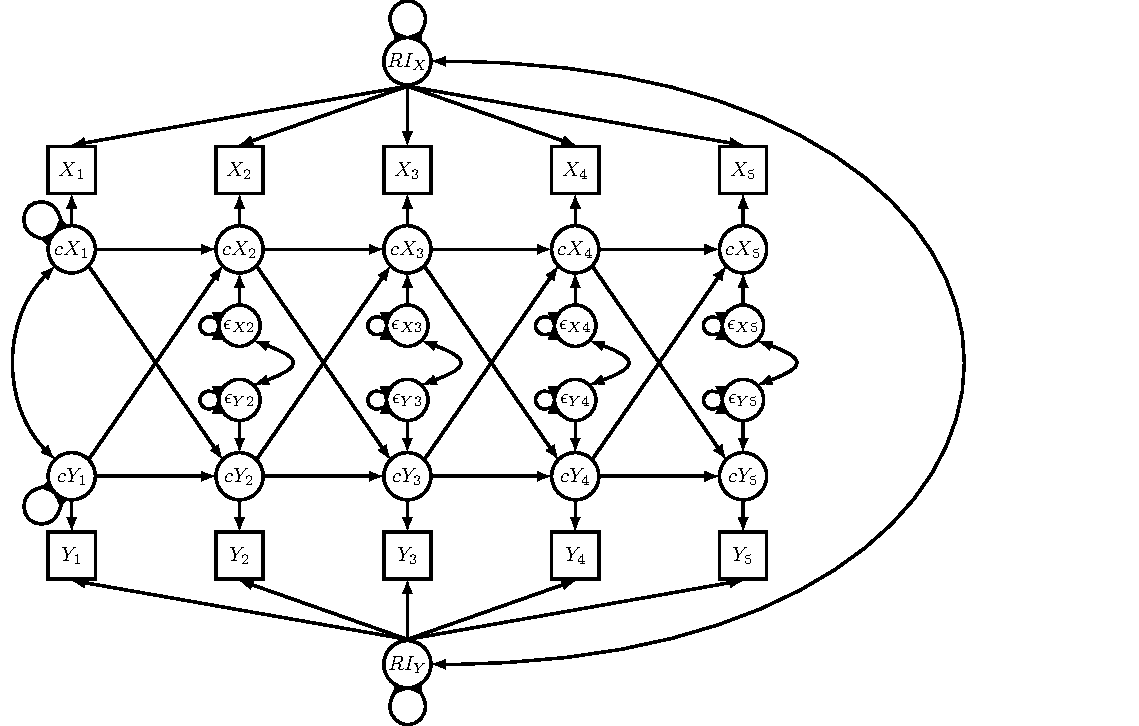
\includegraphics{riclpm_cropped.pdf}

}

}

\subcaption{\label{fig-riclpm}Random Intercept Cross-Lagged Panel Model
(RI-CLPM)}
\end{minipage}%
\newline
\begin{minipage}[t]{\linewidth}

{\centering 

\raisebox{-\height}{

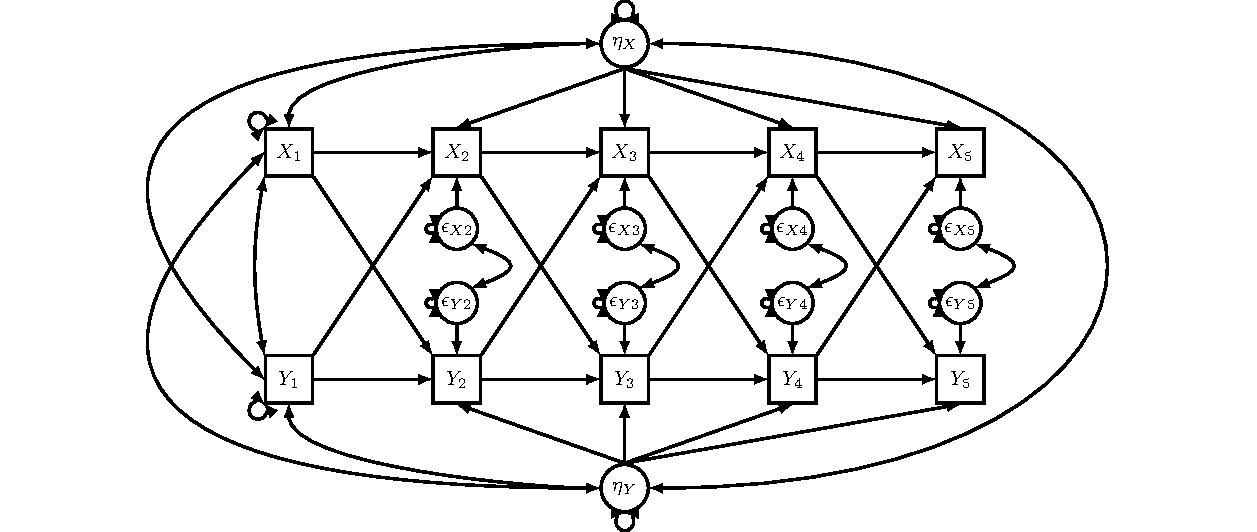
\includegraphics{dpm_cropped.pdf}

}

}

\subcaption{\label{fig-dpm}Dynamic Panel Model (DPM)}
\end{minipage}%

\caption{\label{fig-models}Two Popular Models in Panel Research. Boxes
Indicate Observed Variables and Circles Indicate Latent Variables.}

\end{figure}

Therefore, the effect of time-invariant confounders on both the RI-CLPM
and the DPM should be explored further. The current research report will
evaluate the extent to which unobserved time-invariant confounders
affect the estimates of the RI-CLPM and DPM. I will explore different
types of time-invariant confounders in panel data (i.e.~with time-stable
effects versus time-varying effects) and assess their effects on
estimates of the RI-CLPM and DPM when they are unobserved. This will
serve as a preliminary exploration for the thesis, which will address
the use of causal inference methods such as propensity score adjustment
and inverse probability weighting (e.g. Brown et al., 2021; Vansteelandt
\& Daniel, 2014) to control for observed time-invariant confounders in
the RI-CLPM.

This report is structured as follows. I will start with a conceptual
comparison between the RI-CLPM and the DPM. Then, a hypothetical data
generating mechanism that includes multiple time-invariant confounders
will be introduced and the potential of the RI-CLPM and the DPM to
control for unobserved confounding when this mechanism is true will be
discussed. After this, a simulation study will be performed to assess
the performance of the RI-CLPM and the DPM under the data generating
mechanism. Results and implications will be discussed.

\hypertarget{a-comparison-of-the-ri-clpm-and-the-dpm}{%
\section{A Comparison of the RI-CLPM and the
DPM}\label{a-comparison-of-the-ri-clpm-and-the-dpm}}

The RI-CLPM (Hamaker et al., 2015) is often used with the goal to
separate within person dynamics from stable between person differences.
It decomposes the observed scores of an individual in a stable person
mean (the random intercept representing the `between' part of the model)
and a temporal deviation from that mean (the `within' part of the
model). The model implies only direct effects of the stable trait as
well as no effect of the stable trait of one variable on the observed
scores of the other (other than through its covariance with the other
stable trait factor).

The DPM, however, is usually used when the goal is to model lagged
effects while using a latent factor to control for time-invariant
confounders. It does not explicitly decompose within person dynamics
from stable between person differences, and regresses the observed
scores on each other. The latent factors in the DPM are sometimes called
`accumulating factors' (Usami et al., 2019), as their effects on the
observed variables are both direct, as well as indirect through lagged
relationships between the observed variables themselves. Furthermore, to
account for the fact that measurements are usually sampled at a random
moment in time in an ongoing process, the loading for the first
timepoint is estimated freely (Hamaker, 2005), which is not necessary in
the RI-CLPM.

Hamaker (2005) shows that in specific cases, the RI-CLPM and the DPM are
statistically equivalent and yield equivalent estimates of the lagged
parameters. Specifically, this is the case when lagged parameters are
stable over time and the covariances in the DPM at the first timepoint
are constrained to reflect this (rather than estimated freely). This
also implies that when these conditions hold in a causal model, both the
RI-CLPM and the DPM should recover the true effects.

\hypertarget{example-of-a-data-generating-mechanism}{%
\section{Example of a Data Generating
Mechanism}\label{example-of-a-data-generating-mechanism}}

Consider the causal Directed Acyclic Graph (DAG) in figure
Figure~\ref{fig-scm}. It shows a dynamic process for \(t=1,...,5\)
between time-varying variables \(X\) and \(Y\) and includes
time-invariant confounders \(C_1\) and \(C_2\). This causal DAG does not
yet have parametric assumptions. This DAG is most similar to the dynamic
panel model, as observed values are determined by observed values at
previous timepoints, but it can also be interpreted as only explicitely
modeling the within person process.

\begin{figure}

{\centering 

\usetikzlibrary{positioning}
\usetikzlibrary{arrows}
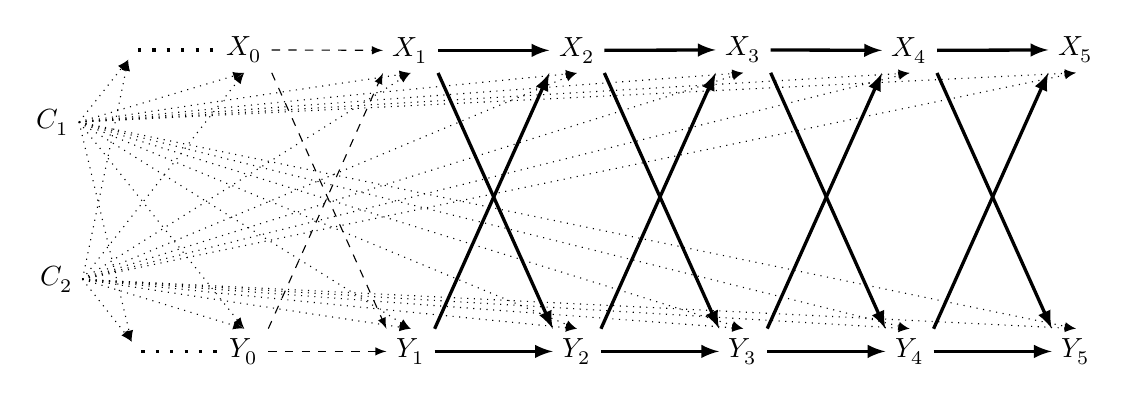
\begin{tikzpicture}[auto,node distance=.5cm, scale=0.5,
paths/.style={->, very thick, -latex},
dot/.style={dotted, ->, -latex},
double/.style={very thick, latex-latex},
dashpath/.style={dashed, ->, -latex}
]
%create nodes
\node (y1) at (0,0) {};
\node[right=1cm of y1] (yt) {$Y_0$};
\node[right=1.5cm of yt] (y2) {$Y_{1}$};
\node[right=1.5cm of y2] (y3){$Y_{2}$};
\node[right=1.5cm of y3] (y4){$Y_{3}$};
\node[right=1.5cm of y4] (y5){$Y_{4}$};
\node[right=1.5cm of y5] (y6){$Y_{5}$};

\node[above=1.5cm of yt] (ut){};
\node[above=1.5cm of y2] (u2){};
\node[above=1.5cm of y3] (u3){};
\node[above=1.5cm of y4] (u4){};
\node[above=1.5cm of y5] (u5){};
\node[above=1.5cm of y6] (u6){};

\node[above=1.5cm of ut] (xt){$X_0$};
\node[left=1cm of xt] (x1){};
\node[above=1.5cm of u2] (x2){$X_{1}$};
\node[above=1.5cm of u3] (x3){$X_{2}$};
\node[above=1.5cm of u4] (x4){$X_{3}$};
\node[above=1.5cm of u5] (x5){$X_{4}$};
\node[above=1.5cm of u6] (x6){$X_{5}$};

\node[below left=0.5cm and 0.5cm of x1] (c1){$C_{1}$};
\node[above left=0.5cm and 0.5cm of y1] (c2){$C_{2}$};

%draw paths
\draw[dashpath] (xt.south east) -- (y2.north west);
\draw[dashpath] (yt.north east) -- (x2.south west);

\draw[paths] (x2.south east) -- (y3.north west);
\draw[paths] (x3.south east) -- (y4.north west);
\draw[paths] (x4.south east) -- (y5.north west);
\draw[paths] (x5.south east) -- (y6.north west);
\draw[paths] (y2.north east) -- (x3.south west);
\draw[paths] (y3.north east) -- (x4.south west);
\draw[paths] (y4.north east) -- (x5.south west);
\draw[paths] (y5.north east) -- (x6.south west);

\draw[loosely dotted, very thick] (x1.east) -- (xt.west);
\draw[dashpath] (xt.east) -- (x2.west);
\draw[paths] (x2.east) -- (x3.west);
\draw[paths] (x3.east) -- (x4.west);
\draw[paths] (x4.east) -- (x5.west);
\draw[paths] (x5.east) -- (x6.west);
\draw[loosely dotted, very thick] (y1.east) -- (yt.west);
\draw[dashpath] (yt.east) -- (y2.west);
\draw[paths] (y2.east) -- (y3.west);
\draw[paths] (y3.east) -- (y4.west);
\draw[paths] (y4.east) -- (y5.west);
\draw[paths] (y5.east) -- (y6.west);

\draw[dot] (c1.east) -- (x1.south);
\draw[dot] (c1.east) -- (xt.south);
\draw[dot] (c1.east) -- (x2.south);
\draw[dot] (c1.east) -- (x3.south);
\draw[dot] (c1.east) -- (x4.south);
\draw[dot] (c1.east) -- (x5.south);
\draw[dot] (c1.east) -- (x6.south);

\draw[dot] (c1.east) -- (y1.north);
\draw[dot] (c1.east) -- (yt.north);
\draw[dot] (c1.east) -- (y2.north);
\draw[dot] (c1.east) -- (y3.north);
\draw[dot] (c1.east) -- (y4.north);
\draw[dot] (c1.east) -- (y5.north);
\draw[dot] (c1.east) -- (y6.north);

\draw[dot] (c2.east) -- (x1.south);
\draw[dot] (c2.east) -- (xt.south);
\draw[dot] (c2.east) -- (x2.south);
\draw[dot] (c2.east) -- (x3.south);
\draw[dot] (c2.east) -- (x4.south);
\draw[dot] (c2.east) -- (x5.south);
\draw[dot] (c2.east) -- (x6.south);

\draw[dot] (c2.east) -- (y1.north);
\draw[dot] (c2.east) -- (yt.north);
\draw[dot] (c2.east) -- (y2.north);
\draw[dot] (c2.east) -- (y3.north);
\draw[dot] (c2.east) -- (y4.north);
\draw[dot] (c2.east) -- (y5.north);
\draw[dot] (c2.east) -- (y6.north);

\end{tikzpicture}

}

\caption{\label{fig-scm}Directed Acyclic Graph for Cross-Lagged
Relationships with 2 Confounders. Dashed Lines Indicate the Process
Before the Observed Timepoints.}

\end{figure}

Assuming the underlying process has been going on for long enough that
it has stabilized around an equilibrium, when lagged effects as well as
the effects of the confounders are time-stable, in both the RI-CLPM and
the DPM the latent factor will be a linear combination of the
confounders (Usami et al., 2019). Therefore, when these conditions hold,
both models should already yield unbiased estimates of the lagged
effects, even when the confounders are unobserved. However, when the
effects of the confounders are not time-stable, the models may not
(fully) take the confounders into account thus resulting in biased
effects. In the next section, a simulation study will be described that
simulates from our DAG and evaluates the performance of the RI-CLPM and
the DPM when confounders are unobserved.

\hypertarget{methods}{%
\section{Methods}\label{methods}}

In previous sections, the RI-CLPM and the DPM have been compared
conceptually and their ability to account for unobserved time-invariant
confounding has been touched upon. In this section, a simulation study
will be presented that evaluates their performance under three different
scenarios. These scenarios are based on the data generating mechanism in
figure Figure~\ref{fig-scm} and differ with respect to the stability of
the effects of the confounders

\hypertarget{data-generation}{%
\subsection{Data Generation}\label{data-generation}}

Below, the different scenarios of the data generating mechanism, that
will be simulated are described, each having different effects of the
confounders. These all follow the following general data generating
mechanism:

For each person \(i\) at timepoint \(t\), \[
x_{it} = \phi_{xx}x_{i,t-1} + \phi_{xy}y_{i,t-1} + \gamma_{1t}C_{1i} + \gamma_{2t}C_{2i} + \epsilon_{xit},
\] \[
y_{it} = \phi_{yy}y_{i,t-1} + \phi_{yx}x_{i,t-1} + \delta_{c1t}C_{i} + \delta_{2t}C_{2i} + \epsilon_{yit}.
\] Furthermore, at the first sampled timepoint, \[
x_{i} = \gamma_{1}C_{1i} + \gamma_{2}C_{2i} + \epsilon_{xi},
\] \[
y_{i} = \delta_{1}C_{1i} + \delta_{2}C_{2i} + \epsilon_{yi}.
\] In addition, \[
\epsilon_{xt} \sim \mathcal{N}(0, \psi_x),
\] \[
\epsilon_{yt} \sim \mathcal{N}(0, \psi_y),
\] \[
C_{1} \sim \mathcal{N}(0, \psi_{C_1}),
\] \[
C_{2} \sim \mathcal{N}(0, \psi_{C_2}).
\]

All lagged effect (cross-lagged effects and autoregressions) and
residual variances will be time-stable, whereas effects of the
confounders may be time-varying. For all scenarios lagged effects are
set to \(\phi_{xx} =\) 0.2, \(\phi_{yy} =\) 0.3, \(\phi_{xy} =\) 0.15,
\(\phi_{yx} =\) 0.1 (based on Mulder, 2023) and the residual variances
are set to \(\psi_x =\) 1, \(\psi_y =\) 1, \(\psi_{C_1} =\) 1, and
\(\psi_{C_2} =\) 1.

Three scenarios will be simulated. For all scenarios, at the start,
\(\gamma_{1} =\) 0.3, \(\gamma_{2} =\) 0.8, \(\delta_{1} =\) 0.5, and
\(\delta_{2} =\) 0.2. For scenario 1, the effects of the confounders
remain stable. For scenario 2, at \(t=3\), the effect of \(C_1\) on
\(x\) and \(y\) decreases and remains stable afterwards,
\(\gamma_{1t} =\) 0.1 and \(\delta_{1t} =\) 0.2. For scenario 3, at
\(t=3\) all effects confounder effects change and afterwards remain
stable \(\gamma_{1t} =\) 0.6 and \(\delta_{1t} =\) 0.2,
\(\gamma_{2t} =\) 0.3 and \(\delta_{2t} =\) 0.5.

1000 datasets are simulated according to each scenario with N=500. To
allow for convergence to an equilibrium, 50 timepoints are simulated, of
which 45 are used as burn-in. The remaining 5 timepoints are used for
analysis.

\hypertarget{analysis}{%
\subsection{Analysis}\label{analysis}}

To assess the performance of the described models when the confounders
are unobserved, all simulated datasets described above will be analyzed
using the RI-CLPM and the DPM, as well as versions of these models with
free factor loadings, as these may, in part, capture some time-varying
heterogeineity due to the confounders. Models that do not converge or do
not result in positive definite covariance matrices will be excluded.
All simulation will be done using R (R Core Team, 2022) and models will
be fit using the lavaan package (Rosseel, 2012).

\hypertarget{results}{%
\section{Results}\label{results}}

Figure~\ref{fig-biases} shows the biases for the \(x_4 \rightarrow y_5\)
effect in scenario 1 and 2. The error bars indicate the Monte Carlo
error, which can be interpreted as the standard error for the bias
estimates (Morris et al., 2019). Scenario 3 is not included in the
results, because all RI-CLPM models and almost all DPM models resulted
in a non positive-definite covariance matrix of the latent variables.

Figure~\ref{fig-biases-1} shows that under scenario 1, as expected, both
the RI-CLPM and the DPM yield unbiased estimates. Surprisingly, freeing
the factor loadings, however, results in bias. Specifically, they yield
a negative bias, indicating that they underestimate the effect.
Furthermore, the RI-CLPM has an MSE of 0.0032663 and the DPM has an MSE
of 0.0019128, indicating that under this scenario, the DPM may be a
better choice.

Under scenario 2, where the effects one of the confounders is
time-varying, both the RI-CLPM and the DPM yield biased effects.
Furthermore, freeing the factor loadings does not seem to capture the
time-varying effects of the confounders. Furthermore, the RI-CLPM has an
MSE of 0.0060792 and the DPM has an MSE of 0.0019639 under this
scenario.

\begin{figure}

\begin{minipage}[t]{\linewidth}

{\centering 

\raisebox{-\height}{

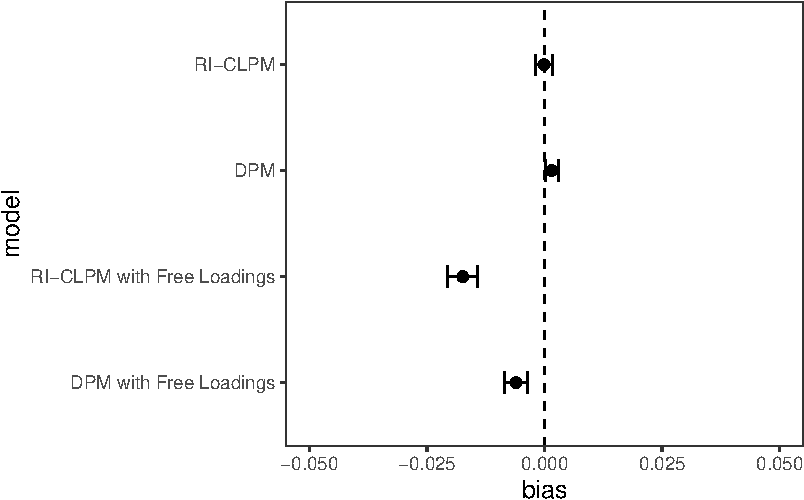
\includegraphics{research-report_files/figure-pdf/fig-biases-1.pdf}

}

}

\subcaption{\label{fig-biases-1}Scenario 1: Time-Stable Effects}
\end{minipage}%
\newline
\begin{minipage}[t]{\linewidth}

{\centering 

\raisebox{-\height}{

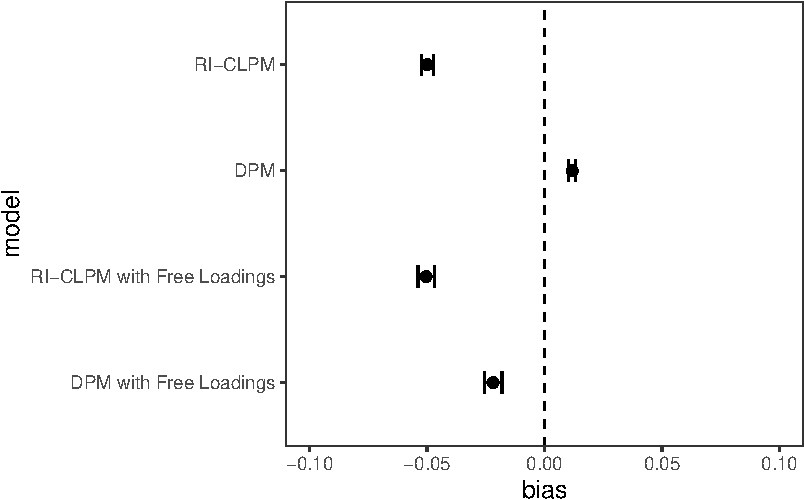
\includegraphics{research-report_files/figure-pdf/fig-biases-2.pdf}

}

}

\subcaption{\label{fig-biases-2}Scenario 2: Time-Varying Effects for C1,
Time-Stable Effects for C2}
\end{minipage}%

\caption{\label{fig-biases}Biases for Scenario 1 and Scenario 2. The
dots indicate the bias of the models and the error bars indicate the
Monte Carlo Error}

\end{figure}

\hypertarget{discussion}{%
\section{Discussion}\label{discussion}}

Pearl \& Mackenzie (2019) argue that science has been in a `causal
revolution' and as Haber et al. (2022) shows, there is an abundance of
causal language present in modern research. It is therefore essential
that causal effects are estimated with great care. Evaluating causality
using reciprocal effects in longitudinal data can bring researchers in
the social science one step closer to obtaining the `true' causal
effect, but more will be necessary.

It has been known that when lagged effects as well as the effect of
unobserved time-invariant confounders are stable over time, both the
RI-CLPM and the DPM can recover the true effect. This characteristic of
both models was replicated by the discussed simulations. However, the
extent to which this is a reasonable causal model is debatable. For many
phenomena, it may be more realistic to assume effects of confounders to
vary over time. Furthermore, when times between measurements are not
equal, time-stable lagged effect cannot be assumed either.

It is therefore necessary to expand the toolbox of social science
researchers by investigating the use of causal inference methods in
cross-lagged panel models, which will be covered by the thesis. The
presented results show the necessity of such techniques and highlight
the importance of acting with cause when attempting to assess cause and
effect.

\newpage{}

\hypertarget{references}{%
\section*{References}\label{references}}
\addcontentsline{toc}{section}{References}

\hypertarget{refs}{}
\begin{CSLReferences}{1}{0}
\leavevmode\vadjust pre{\hypertarget{ref-brown2021}{}}%
Brown, D. W., Greene, T. J., Swartz, M. D., Wilkinson, A. V., \&
DeSantis, S. M. (2021). Propensity score stratification methods for
continuous treatments. \emph{Statistics in Medicine}, \emph{40}(5),
1189--1203. \url{https://doi.org/10.1002/sim.8835}

\leavevmode\vadjust pre{\hypertarget{ref-haber2022}{}}%
Haber, N. A., Wieten, S. E., Rohrer, J. M., Arah, O. A., Tennant, P. W.
G., Stuart, E. A., Murray, E. J., Pilleron, S., Lam, S. T., Riederer,
E., Howcutt, S. J., Simmons, A. E., Leyrat, C., Schoenegger, P., Booman,
A., Dufour, M.-S. K., O'Donoghue, A. L., Baglini, R., Do, S., \ldots{}
Fox, M. P. (2022). Causal and {Associational Language} in {Observational
Health Research}: {A Systematic Evaluation}. \emph{American Journal of
Epidemiology}, \emph{191}(12), 2084--2097.
\url{https://doi.org/10.1093/aje/kwac137}

\leavevmode\vadjust pre{\hypertarget{ref-hamaker2005}{}}%
Hamaker, E. L. (2005). Conditions for the {Equivalence} of the
{Autoregressive Latent Trajectory Model} and a {Latent Growth Curve
Model With Autoregressive Disturbances}. \emph{Sociological Methods \&
Research}, \emph{33}(3), 404--416.
\url{https://doi.org/10.1177/0049124104270220}

\leavevmode\vadjust pre{\hypertarget{ref-hamaker2015}{}}%
Hamaker, E. L., Kuiper, R. M., \& Grasman, R. P. P. P. (2015). A
critique of the cross-lagged panel model. \emph{Psychological Methods},
\emph{20}(1), 102--116. \url{https://doi.org/10.1037/a0038889}

\leavevmode\vadjust pre{\hypertarget{ref-morris2019}{}}%
Morris, T. P., White, I. R., \& Crowther, M. J. (2019). Using simulation
studies to evaluate statistical methods. \emph{Statistics in Medicine},
\emph{38}(11), 2074--2102. \url{https://doi.org/10.1002/sim.8086}

\leavevmode\vadjust pre{\hypertarget{ref-mulder2023}{}}%
Mulder, J. D. (2023). Power {Analysis} for the {Random Intercept
Cross-Lagged Panel Model Using} the {powRICLPM R-Package}.
\emph{Structural Equation Modeling: A Multidisciplinary Journal},
\emph{30}(4), 645--658.
\url{https://doi.org/10.1080/10705511.2022.2122467}

\leavevmode\vadjust pre{\hypertarget{ref-mulder2021}{}}%
Mulder, J. D., \& Hamaker, E. L. (2021). Three {Extensions} of the
{Random Intercept Cross-Lagged Panel Model}. \emph{Structural Equation
Modeling: A Multidisciplinary Journal}, \emph{28}(4), 638--648.
\url{https://doi.org/10.1080/10705511.2020.1784738}

\leavevmode\vadjust pre{\hypertarget{ref-murayama2022}{}}%
Murayama, K., \& Gfrörer, T. (2022). \emph{Thinking clearly about
time-invariant confounders in cross-lagged panel models: {A} guide for
choosing a statistical model from a causal inference perspective}
{[}Preprint{]}. {PsyArXiv}.

\leavevmode\vadjust pre{\hypertarget{ref-pearl2019}{}}%
Pearl, J., \& Mackenzie, D. (2019). \emph{The {Book} of {Why}: {The New
Science} of {Cause} and {Effect}}. {Penguin Books UK}.

\leavevmode\vadjust pre{\hypertarget{ref-R}{}}%
R Core Team. (2022). \emph{R: {A Language} and {Environment} for
{Statistical Computing}}. {R Foundation for Statistical Computing}.

\leavevmode\vadjust pre{\hypertarget{ref-lavaan}{}}%
Rosseel, Y. (2012). \{Lavaan\}: {An} \{\vphantom\}{R}\vphantom\{\}
{Package} for {Structural Equation Modeling}. \emph{Journal of
Statistical Software}, \emph{48}(2), 1--36.
\url{https://doi.org/10.18637/jss.v048.i02}

\leavevmode\vadjust pre{\hypertarget{ref-usami2019}{}}%
Usami, S., Murayama, K., \& Hamaker, E. L. (2019). A unified framework
of longitudinal models to examine reciprocal relations.
\emph{Psychological Methods}, \emph{24}(5), 637--657.
\url{https://doi.org/10.1037/met0000210}

\leavevmode\vadjust pre{\hypertarget{ref-vansteelandt2014}{}}%
Vansteelandt, S., \& Daniel, R. m. (2014). On regression adjustment for
the propensity score. \emph{Statistics in Medicine}, \emph{33}(23),
4053--4072. \url{https://doi.org/10.1002/sim.6207}

\end{CSLReferences}



\end{document}
